% This file was created by tikzplotlib v0.9.8.
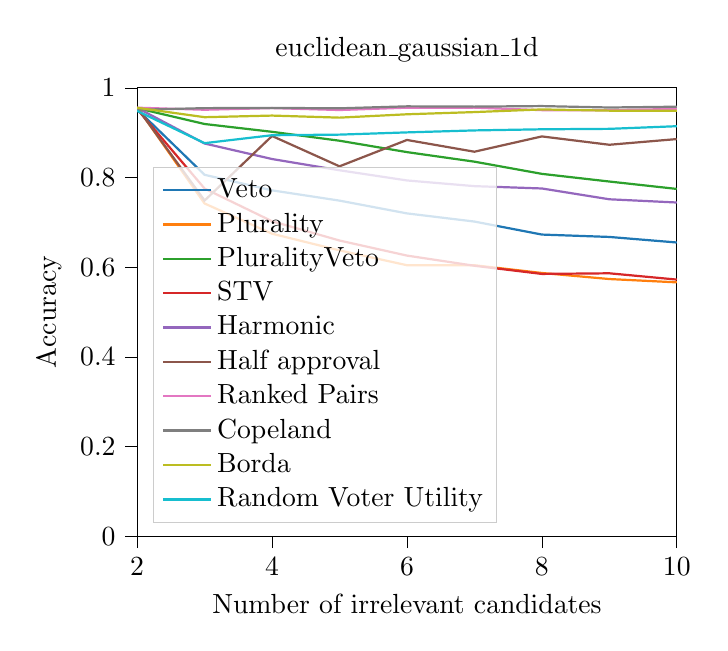
\begin{tikzpicture}

\definecolor{color0}{rgb}{0.12156862745098,0.466666666666667,0.705882352941177}
\definecolor{color1}{rgb}{1,0.498039215686275,0.0549019607843137}
\definecolor{color2}{rgb}{0.172549019607843,0.627450980392157,0.172549019607843}
\definecolor{color3}{rgb}{0.83921568627451,0.152941176470588,0.156862745098039}
\definecolor{color4}{rgb}{0.580392156862745,0.403921568627451,0.741176470588235}
\definecolor{color5}{rgb}{0.549019607843137,0.337254901960784,0.294117647058824}
\definecolor{color6}{rgb}{0.890196078431372,0.466666666666667,0.76078431372549}
\definecolor{color7}{rgb}{0.737254901960784,0.741176470588235,0.133333333333333}
\definecolor{color8}{rgb}{0.0901960784313725,0.745098039215686,0.811764705882353}

\begin{axis}[
legend cell align={left},
legend style={
  fill opacity=0.8,
  draw opacity=1,
  text opacity=1,
  at={(0.03,0.03)},
  anchor=south west,
  draw=white!80!black
},
tick align=outside,
tick pos=left,
title={euclidean\_gaussian\_1d},
x grid style={white!69.0196078431373!black},
xlabel={Number of irrelevant candidates},
xmin=2, xmax=10,
xtick style={color=black},
y grid style={white!69.0196078431373!black},
ylabel={Accuracy},
ymin=0, ymax=1,
ytick style={color=black}
]
\addplot [thick, color0]
table {%
2 0.952
3 0.8061
4 0.7714
5 0.7485
6 0.72
7 0.7018
8 0.6728
9 0.6675
10 0.6551
};
\addlegendentry{Veto}
\addplot [thick, color1]
table {%
2 0.957
3 0.7421
4 0.6747
5 0.6375
6 0.6044
7 0.6044
8 0.5871
9 0.5736
10 0.5662
};
\addlegendentry{Plurality}
\addplot [thick, color2]
table {%
2 0.9547
3 0.9194
4 0.902
5 0.8821
6 0.8567
7 0.8354
8 0.8082
9 0.7911
10 0.7746
};
\addlegendentry{PluralityVeto}
\addplot [thick, color3]
table {%
2 0.9527
3 0.7754
4 0.7025
5 0.6595
6 0.6259
7 0.6032
8 0.585
9 0.5864
10 0.5724
};
\addlegendentry{STV}
\addplot [thick, color4]
table {%
2 0.9555
3 0.8759
4 0.8413
5 0.8162
6 0.7935
7 0.7808
8 0.7756
9 0.7515
10 0.7443
};
\addlegendentry{Harmonic}
\addplot [thick, color5]
table {%
2 0.9558
3 0.7487
4 0.8927
5 0.825
6 0.8838
7 0.8576
8 0.8917
9 0.8731
10 0.8858
};
\addlegendentry{Half approval}
\addplot [thick, color6]
table {%
2 0.9558
3 0.9512
4 0.9549
5 0.9506
6 0.9558
7 0.9559
8 0.9503
9 0.9502
10 0.9531
};
\addlegendentry{Ranked Pairs}
\addplot [thick, white!49.8039215686275!black]
table {%
2 0.9511
3 0.9548
4 0.9553
5 0.9544
6 0.9588
7 0.9582
8 0.9594
9 0.9562
10 0.958
};
\addlegendentry{Copeland}
\addplot [thick, color7]
table {%
2 0.9556
3 0.9346
4 0.9382
5 0.9336
6 0.9411
7 0.946
8 0.9519
9 0.9492
10 0.9489
};
\addlegendentry{Borda}
\addplot [thick, color8]
table {%
2 0.9486
3 0.8767
4 0.8944
5 0.8957
6 0.9007
7 0.9051
8 0.9076
9 0.9086
10 0.9145
};
\addlegendentry{Random Voter Utility}
\end{axis}

\end{tikzpicture}
